\documentclass{article}
\usepackage[utf8]{inputenc}
\usepackage{amsmath}
\usepackage{graphicx}
\graphicspath{{.}}

\title{401 HW 1}
\author{James Oswald}
\date{September 2020}

\begin{document}

\maketitle

\section{}
\subsection{Calculus, Taylor series}
Consider the function $f(x)=\frac{\sin(x)}{x}$.
\subsubsection{}
Compute the limit $\lim_{x\to0}f(x)$ using l’Hopital’s rule.
\\\\
\newline
l’Hopital’s rule states that when $\lim_{x\to c}a(x) = \lim_{x\to c}b(x) = 0$ or $\pm\infty$:
\[\lim_{x\to c}\frac{a(x)}{b(x)} = \lim_{x\to c}\frac{a'(x)}{b'(x)}\]
Therefore since the preconditions are met:
\[\lim_{x\to 0}\sin(x) = 0\]
\[\lim_{x\to 0} x = 0\]
We can apply l’Hopital’s rule and get:
\[\lim_{x\to 0}f(x)=\lim_{x\to 0}\frac{\sin(x)}{x}=\lim_{x\to 0}\frac{\cos(x)}{1}\]
Since:
\[(\sin(x))' = \cos(x) \newline\]
\[(x)' = 1\]
Evaluating we get:
\[\lim_{x\to 0}\frac{\cos(x)}{1} = \lim_{x\to 0}\cos(x) = 1\]
Therefore:
\[\lim_{x\to0}f(x) = 1\]

\subsubsection{}
Use Taylor’s remainder theorem to get the same result:
\paragraph{a)} Write down $P_1(x)$, the first-order Taylor polynomial for $\sin(x)$ centered at $a = 0$.
\\\\
By definition, a first order Taylor polynomial for a function $f(x)$ centered at $a$ takes the form:
\[P_1(x) = f(a) + f'(a)(x-a)\]
So we get that for $\sin(x)$ at $a = 0$:
\begin{equation}
\begin{aligned}
P_1(x) &= \sin(0) + \cos(0)(x - 0) \\
&= 0 + 1x \\
&= x\\
\nonumber
\end{aligned}
\end{equation}
Therefore:
\[P_1(x) = x\] 

\paragraph{b)} Write down a good upper bound on the absolute value of the remainder $R_1(x) = \sin(x)-P_1(x)$, using your knowledge about the derivatives of $sin(x)$. The goal here is to show that $R_1(x)/x$ is negligible.
\\\\
By definition, the remainder is:
\[R_n(x)=\frac{f^{n+1}(a)}{(n+1)!}(x-a)^{n+1}\]
Since in this case $n=1$, $a=0$, and $f(x)=\sin(x)$ we get:
\begin{equation}
\begin{aligned}
R_1(x)&=\frac{f''(0)}{2!}x^2\\
&=\frac{-\sin(0)}{2}x^2\\
&=\frac{0}{2}x^2\\
&=0\\
\nonumber
\end{aligned}
\end{equation}
Thus, the upper bound of the remainder is 0, and we have shown that $R_1(x)/x$ is negligible since:
\[0/x = 0 \;\;\text{when}\;\; x\to 0\] 

\paragraph{c)} Express $f(x)$ as $f(x) = \frac{P_1(x)}{x} + \frac{R_1(x)}{x}$, and compute the limits of the two terms as $x\to0$.
\\\\
By our previous calculations of $P_1(x)$ and $R_1(x)$ we get:
\[\frac{\sin(x)}{x} = \frac{x}{x} + \frac{0}{x}\]
Now applying limit rules and taking the limit of both sides we get:
\begin{equation}
\begin{aligned}
\lim_{x\to 0}\frac{\sin(x)}{x} &= \lim_{x\to 0}\left(\frac{x}{x} + \frac{0}{x}\right)\\
&= \lim_{x\to 0}\frac{x}{x} + \lim_{x\to 0}\frac{0}{x}\\
&= 1 + 0\\
&= 1\\
\nonumber
\end{aligned}
\end{equation}
Thus:
\[\lim_{x\to 0}\frac{\sin(x)}{x} = 1\]
Which is the same result as derived by using l’Hopital’s rule.


\subsection{Asymptotic notation}
Recall the definitions of the asymptotic notations. We will say that $f(x)$ has "order of growth $x^\alpha$ as $x\to x_0$" (where $x_0$ is either some fixed real number or $\pm\infty$) if $f(x) = \Theta(x^\alpha)$ as $x\to x_0$.

\subsubsection{}
Consider the functions $f(x) = x \sin(x)$ and $g(x) = x$. Is $f(x) = \Theta(g(x))$ as $x\to \infty$? Why or
why not? (Hint: As always, you should refer back carefully to the definition of $\Theta(\cdot)$.)
\\\\
By definition of Big Theta, $f(x) = \Theta(g(x))$ iff:
\[\lim_{x\to\infty}\frac{f(x)}{g(x)} = c \;\;\text{and}\;\; 0 < c < \infty\]
In our case we have $f(x) = x \sin(x)$ and $g(x) = x$ so:
\[\lim_{x\to\infty}\frac{x\sin(x)}{x}\]
\[\lim_{x\to\infty}\sin(x)\]
But we know that:
\[\lim_{x\to\infty}\sin(x) = \text{DNE}\]
and since its DNE, no c exists between 0 and $\infty$. Therefore $f(x)$ is not $\Theta(g(x))$

\subsubsection{}
Suppose that we know that $f(x) = x + \Theta(x^2)$ and $g(x) = \Theta(x) > 0$ as $x\to 0$. Determine the order of growth of $f(x) + g(x)$.\\ (This problem is meant to get you comfortable with manipulating asymptotic notation when it appears in expressions. When I say something like "$f(x) = x + \Theta(x^2)$", this means that there is some function $h(x) = \Theta(x^2)$, and $f(x) = x+h(x)$. That is, the fact that $h(x) = \Theta(x^2)$ is the only thing you know about $h(x)$.)
\\\\
First expanding $f(x) + g(x)$ we see:
\[f(x) + g(x) = x + \Theta(x^2) + g(x)\]
We know that this means there exists some function $h(x) = \Theta(x^2)$. As $x\to 0$ the $g(x)$ term which is $\Theta(x)$ dominates the unknown $h(x)$ term which is $\Theta(x^2)$, meaning the order of growth of $f(x) + g(x)$ as $x\to 0$ will be $\Theta(x)$.

\subsubsection{}
Suppose that we know that $f(x) = e^{\Theta(x)}$ as $x\to\infty$. Does this imply that $f(x) = \Theta(e^x)$? (Hint: Think carefully about the definition of $\Theta(\cdot)$, and consider $f(x) = e^{2x}$.)
\\\\
By the definition of $\Theta(\cdot)$, we see that $f(x) = e^{\Theta(x)}$ implies there exists constants $c_1$ and $c_2$ such that:
\[e^{c_1\cdot x} \leq f(x) \leq e^{c_2 \cdot x}\]
we see that for any $c_1$ and $c_2$, $f(x)$ is still bounded by $\Theta(e^x)$ on both sides, therefore $f(x) = \Theta(e^x)$

\subsection{Relative versus absolute error}

\subsubsection{}
Suppose that you are approximating a function $g(n)$ by some function $f(n)$. Suppose, further, that you know that the absolute error in approximating $g(n)$ by $f(n)$ satisfies $|f(n)-g(n)| = o(1)$ as $n\to \infty$ (that is, $\lim_{n\to\infty} |f(n) - g(n)| = 0$). Is it true that the relative error also decays to 0? If not, come up with functions $f(n)$ and $g(n)$ for which this is not true. (Hint: Come up with some $g(n)$ and $f(n)$ satisfying $g(n) = o(1)$ and $f(n)/g(n) = \Theta(1)$.)
\\\\
Let $f(x) = \frac{1}{n}$ and let $g(x) = \frac{1}{3n}$ both are $o(1)$. These functions satisfy the constraint of having absolute error approach 0 when approximating $g(x)$ with $f(x)$:
\[\lim_{n\to\infty} |f(n) - g(n)| = \lim_{n\to\infty}\left|\frac{1}{n} - \frac{1}{3n}\right| = \lim_{n\to\infty}\frac{2}{3n} = 0\]
However, when computing the relative error we find:
\[\frac{\frac{2}{3n}}{\frac{1}{3n}} = 2\]
and since:
\[\lim_{n\to\infty}2 = 2\]
we see that the relative error doesn't decay to 0, but rather stays constant. 

\subsection{Matlab warmup/Gentle linear algebra review}

\subsubsection{Exercise 2}
See the attached diary file for MATLAB results

$A = \begin{pmatrix}10 & -3\\4&2\end{pmatrix}$, $B = \begin{pmatrix}1 & 0\\-1&2\end{pmatrix}$, $v = \begin{pmatrix}1\\2\end{pmatrix}$, $w = \begin{pmatrix}1\\1\end{pmatrix}$
\paragraph{a)}
\[v^Tw = \begin{pmatrix}1\\2\end{pmatrix}^T\begin{pmatrix}1\\1\end{pmatrix} = \begin{pmatrix}1&2\end{pmatrix}\begin{pmatrix}1\\1\end{pmatrix} = \begin{pmatrix}1\cdot1+2\cdot1\end{pmatrix} = \begin{pmatrix}3\end{pmatrix}\]
\paragraph{b)}
\[vw^T = \begin{pmatrix}1\\2\end{pmatrix}\begin{pmatrix}1\\1\end{pmatrix}^T = \begin{pmatrix}1\\2\end{pmatrix}\begin{pmatrix}1&1\end{pmatrix} = \begin{pmatrix}1\cdot1&1\cdot1\\2\cdot1&2\cdot1\end{pmatrix} = \begin{pmatrix}1&1\\2&2\end{pmatrix}\]
\paragraph{c)}
\[Av = \begin{pmatrix}10 & -3\\4&2\end{pmatrix}\begin{pmatrix}1\\2\end{pmatrix} = \begin{pmatrix}4\\8\end{pmatrix}\]
\paragraph{d)}
\[A^Tv = \begin{pmatrix}10 & -3\\4&2\end{pmatrix}^T\begin{pmatrix}1\\2\end{pmatrix} = \begin{pmatrix}10 & 4\\-3&2\end{pmatrix}\begin{pmatrix}1\\2\end{pmatrix} = \begin{pmatrix}18\\1\end{pmatrix}\]
\paragraph{e)}
\[AB = \begin{pmatrix}10 & -3\\4&2\end{pmatrix}\begin{pmatrix}1 & 0\\-1&2\end{pmatrix} = \begin{pmatrix}13 & -6\\2&4\end{pmatrix}\]
\paragraph{f)}
\[BA = \begin{pmatrix}1 & 0\\-1&2\end{pmatrix}\begin{pmatrix}10 & -3\\4&2\end{pmatrix} = \begin{pmatrix}10 & -3\\-2&7\end{pmatrix}\]
\paragraph{g)}
\[A^2 = \begin{pmatrix}10 & -3\\4&2\end{pmatrix}\begin{pmatrix}10 & -3\\4&2\end{pmatrix} = \begin{pmatrix}88& -36\\48&-8\end{pmatrix}\]
\paragraph{h)}
The vector $y$ for which $By = w$
\[y = B^{-1}w = \begin{pmatrix}1 & 0\\-1&2\end{pmatrix}^{-1}\begin{pmatrix}1\\1\end{pmatrix} = \begin{pmatrix}1 & 0\\0.5&0.5\end{pmatrix}\begin{pmatrix}1\\1\end{pmatrix} = \begin{pmatrix}1\\1\end{pmatrix}\]
\paragraph{i)}
The vector $x$ for which $Ax = v$
\[x = A^{-1}v = \begin{pmatrix}10&-3\\4&2\end{pmatrix}^{-1}\begin{pmatrix}1\\2\end{pmatrix} = \begin{pmatrix}\frac{1}{16} &\frac{3}{32}\\-\frac{1}{8}&\frac{5}{16}\end{pmatrix}\begin{pmatrix}1\\2\end{pmatrix} = \begin{pmatrix}\frac{1}{4}\\\frac{1}{2}\end{pmatrix}\]

\subsubsection{Exercise 3}
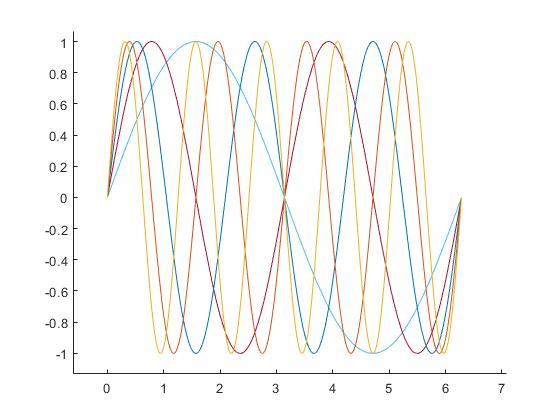
\includegraphics[scale=0.5]{Ex3.jpg}

\end{document}
